% Options for packages loaded elsewhere
% Options for packages loaded elsewhere
\PassOptionsToPackage{unicode}{hyperref}
\PassOptionsToPackage{hyphens}{url}
\PassOptionsToPackage{dvipsnames,svgnames,x11names}{xcolor}
%
\documentclass[
]{article}
\usepackage{xcolor}
\usepackage[margin=2.5cm]{geometry}
\usepackage{amsmath,amssymb}
\setcounter{secnumdepth}{-\maxdimen} % remove section numbering
\usepackage{iftex}
\ifPDFTeX
  \usepackage[T1]{fontenc}
  \usepackage[utf8]{inputenc}
  \usepackage{textcomp} % provide euro and other symbols
\else % if luatex or xetex
  \usepackage{unicode-math} % this also loads fontspec
  \defaultfontfeatures{Scale=MatchLowercase}
  \defaultfontfeatures[\rmfamily]{Ligatures=TeX,Scale=1}
\fi
\usepackage{lmodern}
\ifPDFTeX\else
  % xetex/luatex font selection
\fi
% Use upquote if available, for straight quotes in verbatim environments
\IfFileExists{upquote.sty}{\usepackage{upquote}}{}
\IfFileExists{microtype.sty}{% use microtype if available
  \usepackage[]{microtype}
  \UseMicrotypeSet[protrusion]{basicmath} % disable protrusion for tt fonts
}{}
\makeatletter
\@ifundefined{KOMAClassName}{% if non-KOMA class
  \IfFileExists{parskip.sty}{%
    \usepackage{parskip}
  }{% else
    \setlength{\parindent}{0pt}
    \setlength{\parskip}{6pt plus 2pt minus 1pt}}
}{% if KOMA class
  \KOMAoptions{parskip=half}}
\makeatother
% Make \paragraph and \subparagraph free-standing
\makeatletter
\ifx\paragraph\undefined\else
  \let\oldparagraph\paragraph
  \renewcommand{\paragraph}{
    \@ifstar
      \xxxParagraphStar
      \xxxParagraphNoStar
  }
  \newcommand{\xxxParagraphStar}[1]{\oldparagraph*{#1}\mbox{}}
  \newcommand{\xxxParagraphNoStar}[1]{\oldparagraph{#1}\mbox{}}
\fi
\ifx\subparagraph\undefined\else
  \let\oldsubparagraph\subparagraph
  \renewcommand{\subparagraph}{
    \@ifstar
      \xxxSubParagraphStar
      \xxxSubParagraphNoStar
  }
  \newcommand{\xxxSubParagraphStar}[1]{\oldsubparagraph*{#1}\mbox{}}
  \newcommand{\xxxSubParagraphNoStar}[1]{\oldsubparagraph{#1}\mbox{}}
\fi
\makeatother


\usepackage{longtable,booktabs,array}
\usepackage{calc} % for calculating minipage widths
% Correct order of tables after \paragraph or \subparagraph
\usepackage{etoolbox}
\makeatletter
\patchcmd\longtable{\par}{\if@noskipsec\mbox{}\fi\par}{}{}
\makeatother
% Allow footnotes in longtable head/foot
\IfFileExists{footnotehyper.sty}{\usepackage{footnotehyper}}{\usepackage{footnote}}
\makesavenoteenv{longtable}
\usepackage{graphicx}
\makeatletter
\newsavebox\pandoc@box
\newcommand*\pandocbounded[1]{% scales image to fit in text height/width
  \sbox\pandoc@box{#1}%
  \Gscale@div\@tempa{\textheight}{\dimexpr\ht\pandoc@box+\dp\pandoc@box\relax}%
  \Gscale@div\@tempb{\linewidth}{\wd\pandoc@box}%
  \ifdim\@tempb\p@<\@tempa\p@\let\@tempa\@tempb\fi% select the smaller of both
  \ifdim\@tempa\p@<\p@\scalebox{\@tempa}{\usebox\pandoc@box}%
  \else\usebox{\pandoc@box}%
  \fi%
}
% Set default figure placement to htbp
\def\fps@figure{htbp}
\makeatother





\setlength{\emergencystretch}{3em} % prevent overfull lines

\providecommand{\tightlist}{%
  \setlength{\itemsep}{0pt}\setlength{\parskip}{0pt}}



 


\usepackage{booktabs}
\usepackage{longtable}
\usepackage{array}
\usepackage{multirow}
\usepackage{wrapfig}
\usepackage{float}
\usepackage{colortbl}
\usepackage{pdflscape}
\usepackage{tabu}
\usepackage{threeparttable}
\usepackage{threeparttablex}
\usepackage[normalem]{ulem}
\usepackage{makecell}
\usepackage{xcolor}
\makeatletter
\@ifpackageloaded{caption}{}{\usepackage{caption}}
\AtBeginDocument{%
\ifdefined\contentsname
  \renewcommand*\contentsname{Table of contents}
\else
  \newcommand\contentsname{Table of contents}
\fi
\ifdefined\listfigurename
  \renewcommand*\listfigurename{List of Figures}
\else
  \newcommand\listfigurename{List of Figures}
\fi
\ifdefined\listtablename
  \renewcommand*\listtablename{List of Tables}
\else
  \newcommand\listtablename{List of Tables}
\fi
\ifdefined\figurename
  \renewcommand*\figurename{Figure}
\else
  \newcommand\figurename{Figure}
\fi
\ifdefined\tablename
  \renewcommand*\tablename{Table}
\else
  \newcommand\tablename{Table}
\fi
}
\@ifpackageloaded{float}{}{\usepackage{float}}
\floatstyle{ruled}
\@ifundefined{c@chapter}{\newfloat{codelisting}{h}{lop}}{\newfloat{codelisting}{h}{lop}[chapter]}
\floatname{codelisting}{Listing}
\newcommand*\listoflistings{\listof{codelisting}{List of Listings}}
\makeatother
\makeatletter
\makeatother
\makeatletter
\@ifpackageloaded{caption}{}{\usepackage{caption}}
\@ifpackageloaded{subcaption}{}{\usepackage{subcaption}}
\makeatother
\usepackage{bookmark}
\IfFileExists{xurl.sty}{\usepackage{xurl}}{} % add URL line breaks if available
\urlstyle{same}
\hypersetup{
  pdftitle={HPAI Outbreak: General Epidemic Description},
  colorlinks=true,
  linkcolor={blue},
  filecolor={Maroon},
  citecolor={Blue},
  urlcolor={Blue},
  pdfcreator={LaTeX via pandoc}}


\title{HPAI Outbreak: General Epidemic Description}
\usepackage{etoolbox}
\makeatletter
\providecommand{\subtitle}[1]{% add subtitle to \maketitle
  \apptocmd{\@title}{\par {\large #1 \par}}{}{}
}
\makeatother
\subtitle{Phase 1: December 20, 2025 -- January 13, 2026}
\author{}
\date{2026-02-16}
\begin{document}
\maketitle

\renewcommand*\contentsname{Table of contents}
{
\hypersetup{linkcolor=}
\setcounter{tocdepth}{3}
\tableofcontents
}

\section{Outbreak Overview}\label{outbreak-overview}

As of \textbf{January 13, 2026}, a total of \textbf{103 HPAI-confirmed
outbreaks} have been reported across \textbf{8 counties} and \textbf{59
districts} since the index case on \textbf{December 22, 2025} (22 days).
Both species present in the poultry population (duck, chicken) are
affected. Of the 103 confirmed farms, 51 have completed culling, 11 are
in progress, and 41 are planned.

\section{Distribution by Species and Production
Type}\label{distribution-by-species-and-production-type}

\subsection{Outbreak counts}\label{outbreak-counts}

\begin{longtable}[t]{llccc}

\caption{\label{tbl-species-production}Confirmed HPAI outbreaks by
species and production type, with attack rate relative to total farm
population.}

\tabularnewline

\toprule
Species & Production Type & Total Farms & Outbreaks & Attack Rate (\%)\\
\midrule
Chicken & Broiler 1 & 1248 & 18 & 1.4\\
Chicken & Broiler 2 & 2746 & 56 & 2.0\\
Chicken & Layer & 441 & 7 & 1.6\\
Duck & Conventional & 3691 & 11 & 0.3\\
Duck & Organic & 1034 & 11 & 1.1\\
\addlinespace
\textbf{Chicken} & \textbf{All} & \textbf{4435} & \textbf{81} & \textbf{1.8}\\
\textbf{Duck} & \textbf{All} & \textbf{4725} & \textbf{22} & \textbf{0.5}\\
\textbf{Total} & \textbf{All} & \textbf{9160} & \textbf{103} & \textbf{1.1}\\
\midrule\\
\bottomrule

\end{longtable}

\subsection{Capacity affected}\label{capacity-affected}

\begin{longtable}[t]{llccc}

\caption{\label{tbl-capacity}Estimated animal capacity affected by
species and production type.}

\tabularnewline

\toprule
Species & Production Type & Outbreaks & Total Capacity & Mean Capacity / Farm\\
\midrule
Chicken & Broiler 1 & 18 & 89,916 & 4,995\\
Chicken & Broiler 2 & 56 & 122,505 & 2,188\\
Chicken & Layer & 7 & 125,448 & 17,921\\
Duck & Conventional & 11 & 168,927 & 15,357\\
Duck & Organic & 11 & 9,381 & 853\\
\addlinespace
\textbf{Total} & \textbf{All} & \textbf{103} & \textbf{516,177} & \textbf{5,011}\\
\bottomrule

\end{longtable}

\subsection{Detection method}\label{detection-method}

\begin{longtable}[t]{lccc}

\caption{\label{tbl-detection}Outbreaks by detection method and
species.}

\tabularnewline

\toprule
Species & Contact Tracing & Passive & Preshipment\\
\midrule
Chicken & 1 & 74 & 6\\
Duck & 0 & 22 & 0\\
\textbf{Total} & \textbf{1} & \textbf{96} & \textbf{6}\\
\bottomrule

\end{longtable}

\section{Epidemic Timeline}\label{epidemic-timeline}

\subsection{Daily epidemic curve}\label{daily-epidemic-curve}

\begin{figure}

\centering{

\pandocbounded{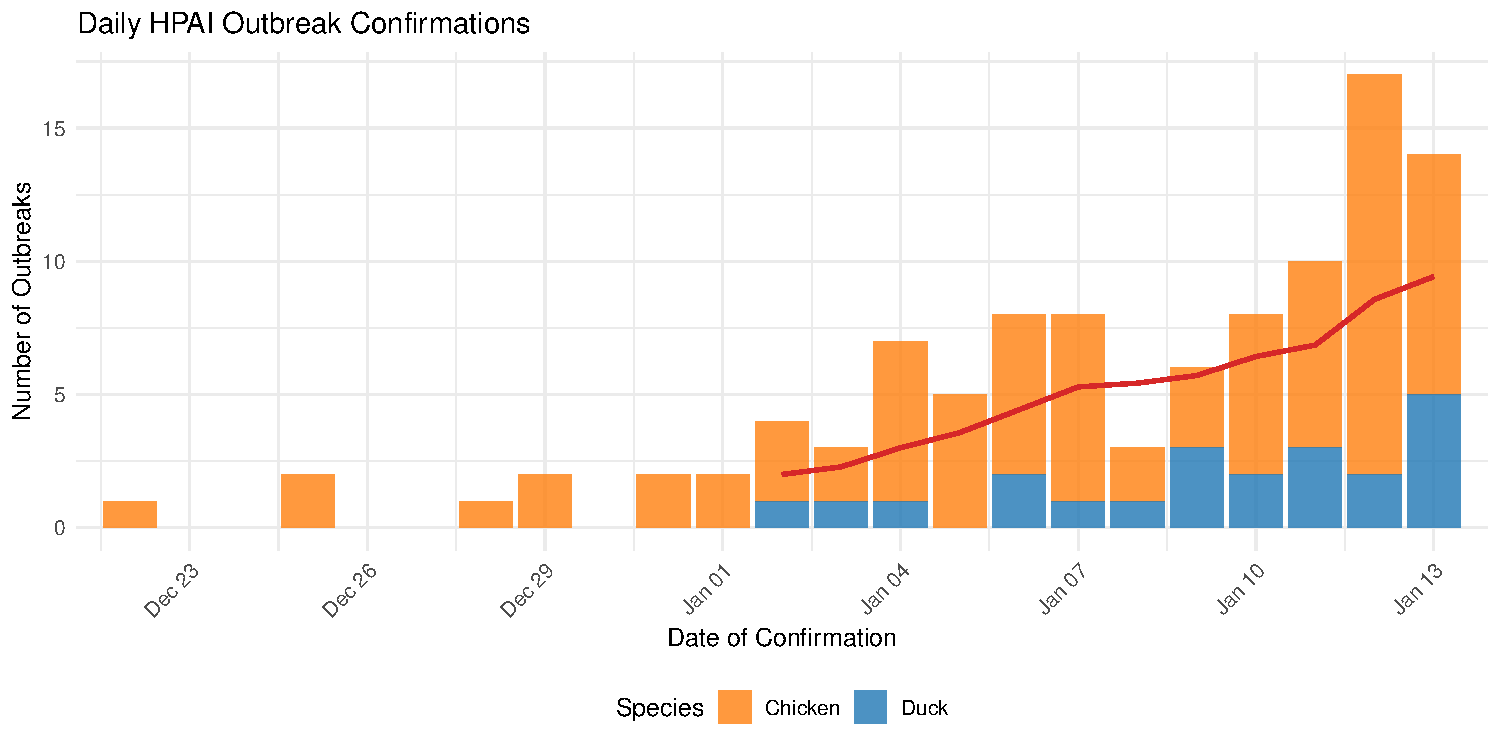
\includegraphics[keepaspectratio]{phase-1-q-1_files/figure-pdf/fig-epicurve-daily-1.pdf}}

}

\caption{\label{fig-epicurve-daily}Daily confirmed HPAI outbreaks (bars)
with 7-day rolling average (red line). Bars are coloured by species.}

\end{figure}%

\subsection{Cumulative epidemic curve}\label{cumulative-epidemic-curve}

\begin{figure}

\centering{

\pandocbounded{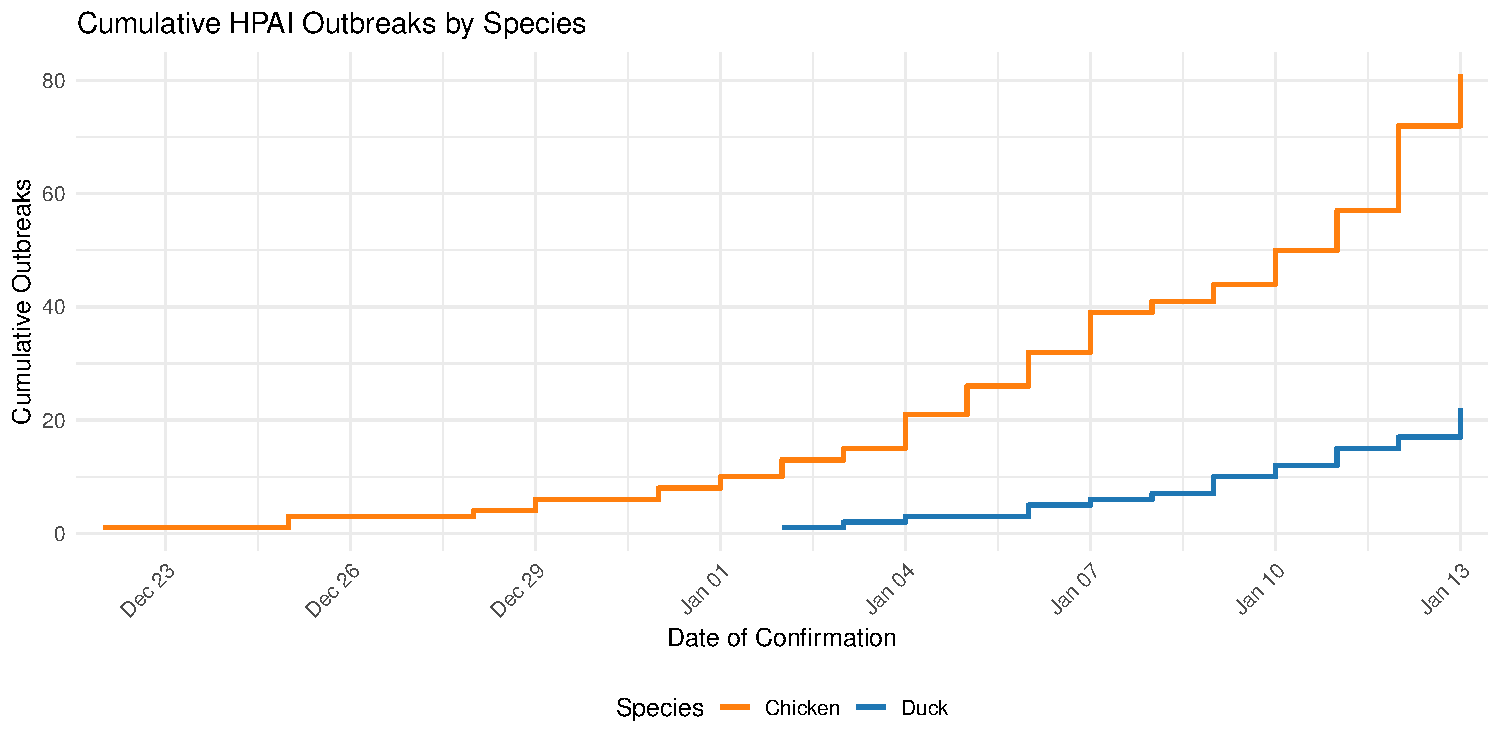
\includegraphics[keepaspectratio]{phase-1-q-1_files/figure-pdf/fig-epicurve-cumulative-1.pdf}}

}

\caption{\label{fig-epicurve-cumulative}Cumulative confirmed HPAI
outbreaks over time, coloured by species.}

\end{figure}%

\subsection{Incidence by epidemiological
week}\label{incidence-by-epidemiological-week}

\begin{longtable}[t]{clcccc}

\caption{\label{tbl-weekly-incidence}Weekly confirmed outbreaks by
species and cumulative total.}

\tabularnewline

\toprule
Week & Period & Duck & Chicken & Week Total & Cumulative\\
\midrule
1 & Dec 22 – Dec 28 & 0 & 4 & 4 & 4\\
2 & Dec 29 – Jan 04 & 3 & 17 & 20 & 24\\
3 & Jan 05 – Jan 11 & 12 & 36 & 48 & 72\\
4 & Jan 12 – Jan 13 & 7 & 24 & 31 & 103\\
\bottomrule

\end{longtable}

\section{Spatial Distribution}\label{spatial-distribution}

\subsection{Outbreak map}\label{outbreak-map}

\begin{figure}

\centering{

\pandocbounded{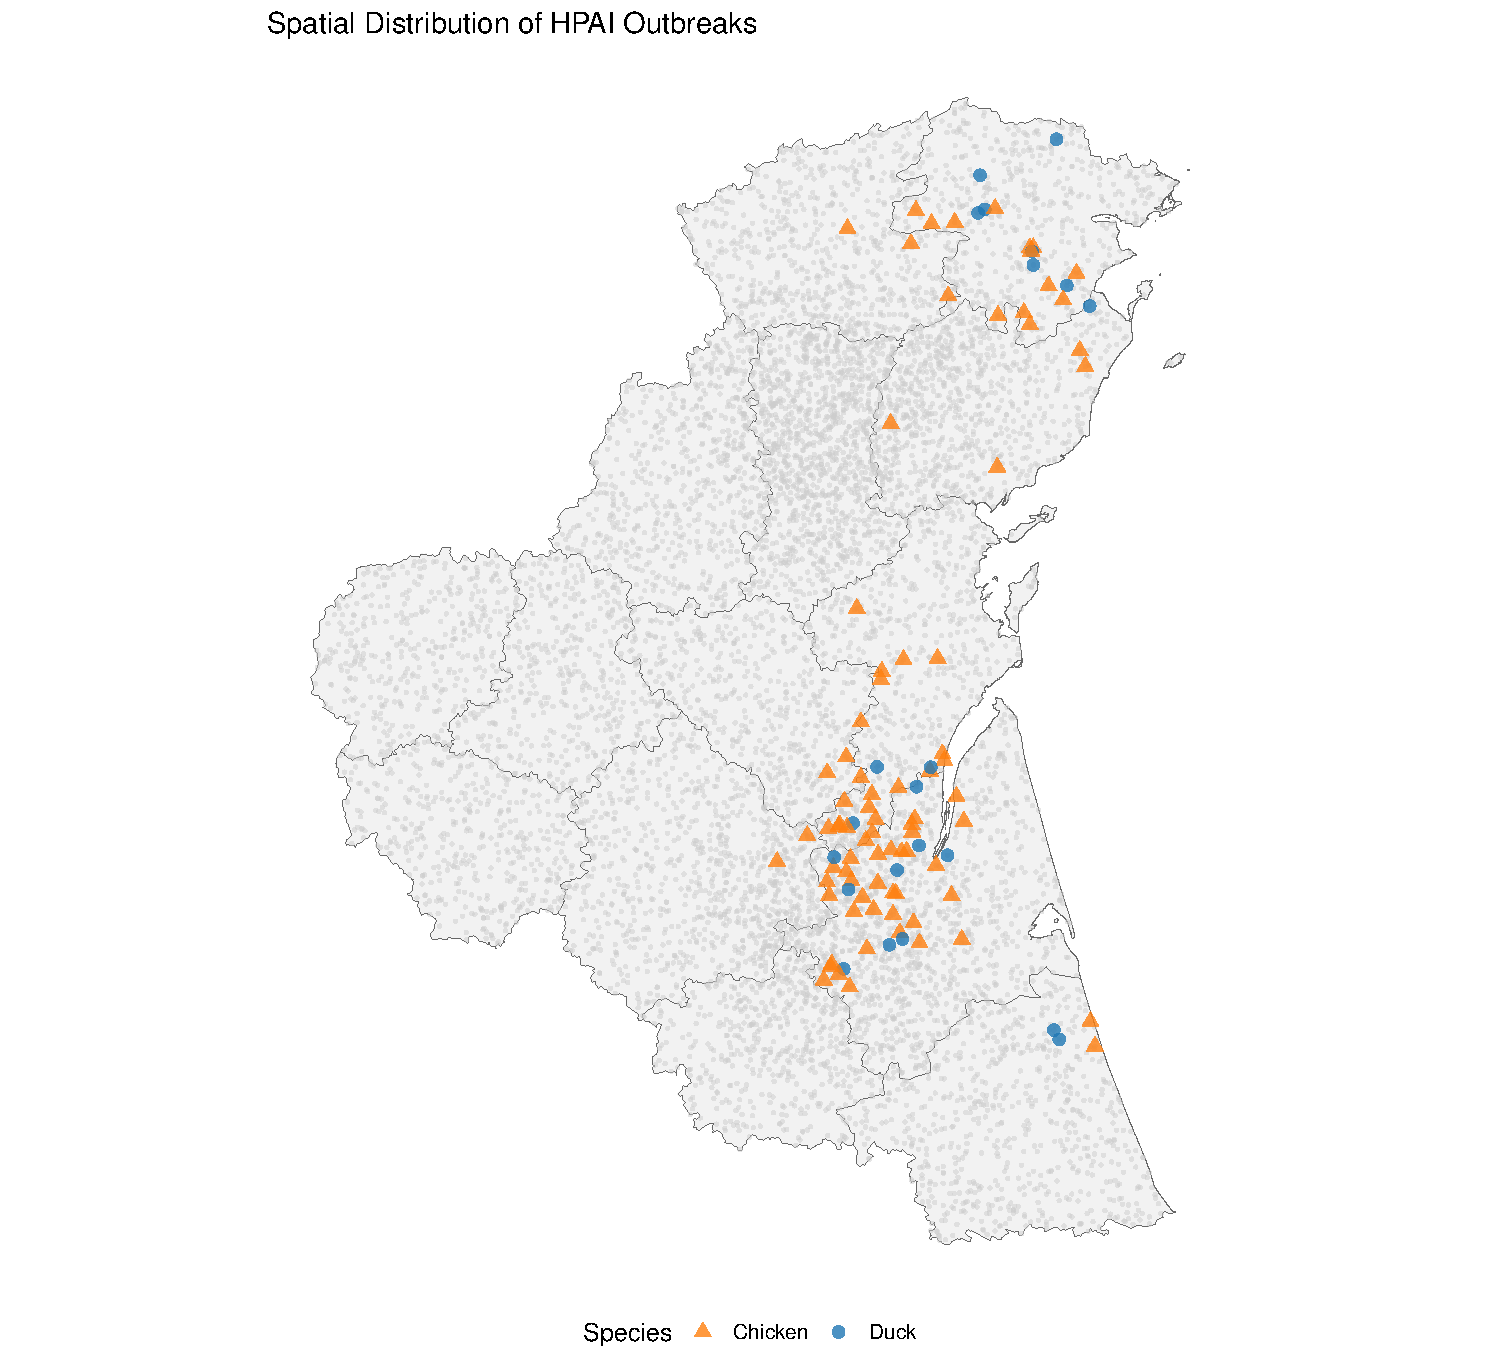
\includegraphics[keepaspectratio]{phase-1-q-1_files/figure-pdf/fig-map-outbreaks-1.pdf}}

}

\caption{\label{fig-map-outbreaks}Spatial distribution of confirmed HPAI
outbreaks (coloured by species) relative to the total farm population
(grey points). County boundaries shown.}

\end{figure}%

\subsection{Outbreaks by county}\label{outbreaks-by-county}

\begin{longtable}[t]{lccc}

\caption{\label{tbl-county}Outbreaks by county, with total farm
population and attack rate.}

\tabularnewline

\toprule
County & Total Farms & Outbreaks & Attack Rate (\%)\\
\midrule
Berks & 1151 & 44 & 3.8\\
Susquehanna & 572 & 22 & 3.8\\
Indiana & 515 & 20 & 3.9\\
Allegheny & 820 & 5 & 0.6\\
Luzerne & 663 & 4 & 0.6\\
\addlinespace
Lancaster & 654 & 3 & 0.5\\
Lycoming & 469 & 3 & 0.6\\
Cumberland & 854 & 2 & 0.2\\
\bottomrule

\end{longtable}

\subsection{Temporal-spatial
progression}\label{temporal-spatial-progression}

\begin{figure}

\centering{

\pandocbounded{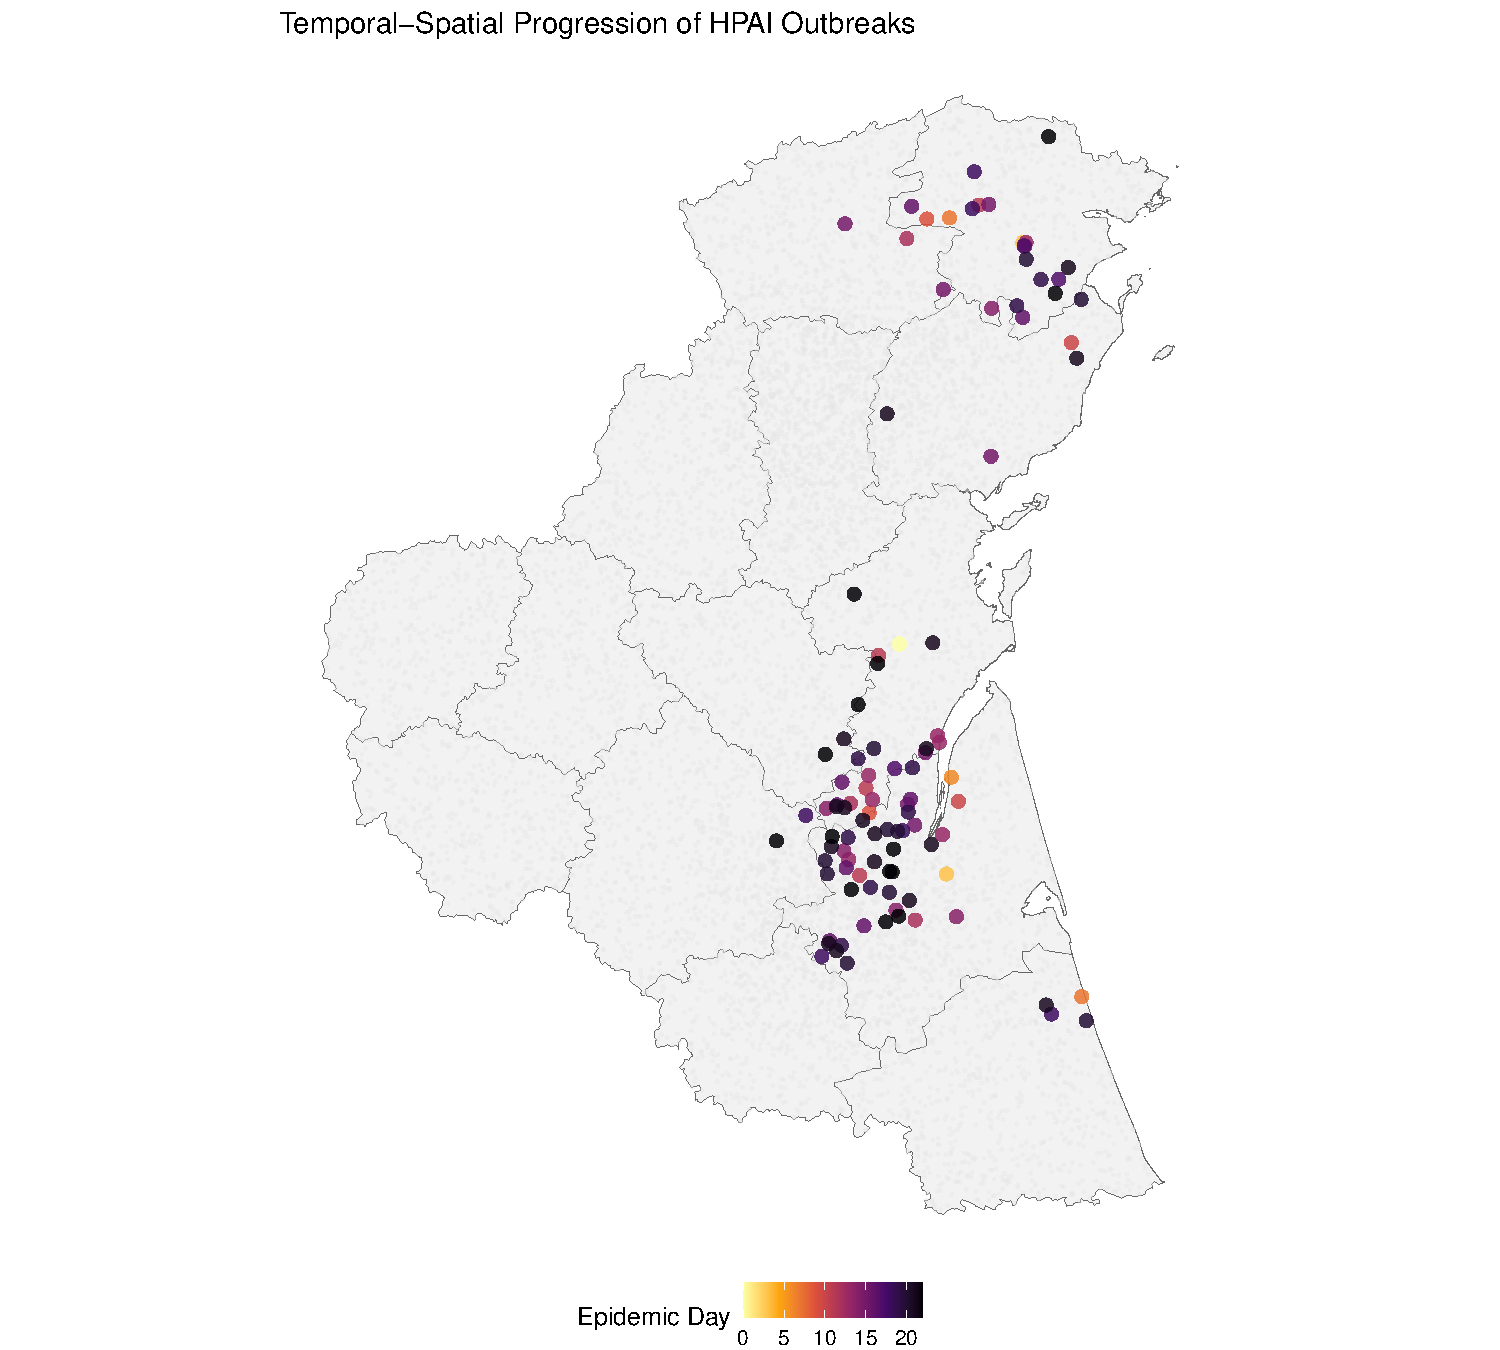
\includegraphics[keepaspectratio]{phase-1-q-1_files/figure-pdf/fig-map-temporal-1.pdf}}

}

\caption{\label{fig-map-temporal}Spatial progression of outbreaks over
time. Point colour indicates timing (darker = earlier). County
boundaries shown for reference.}

\end{figure}%

\subsection{Production type map}\label{production-type-map}

\begin{figure}

\centering{

\pandocbounded{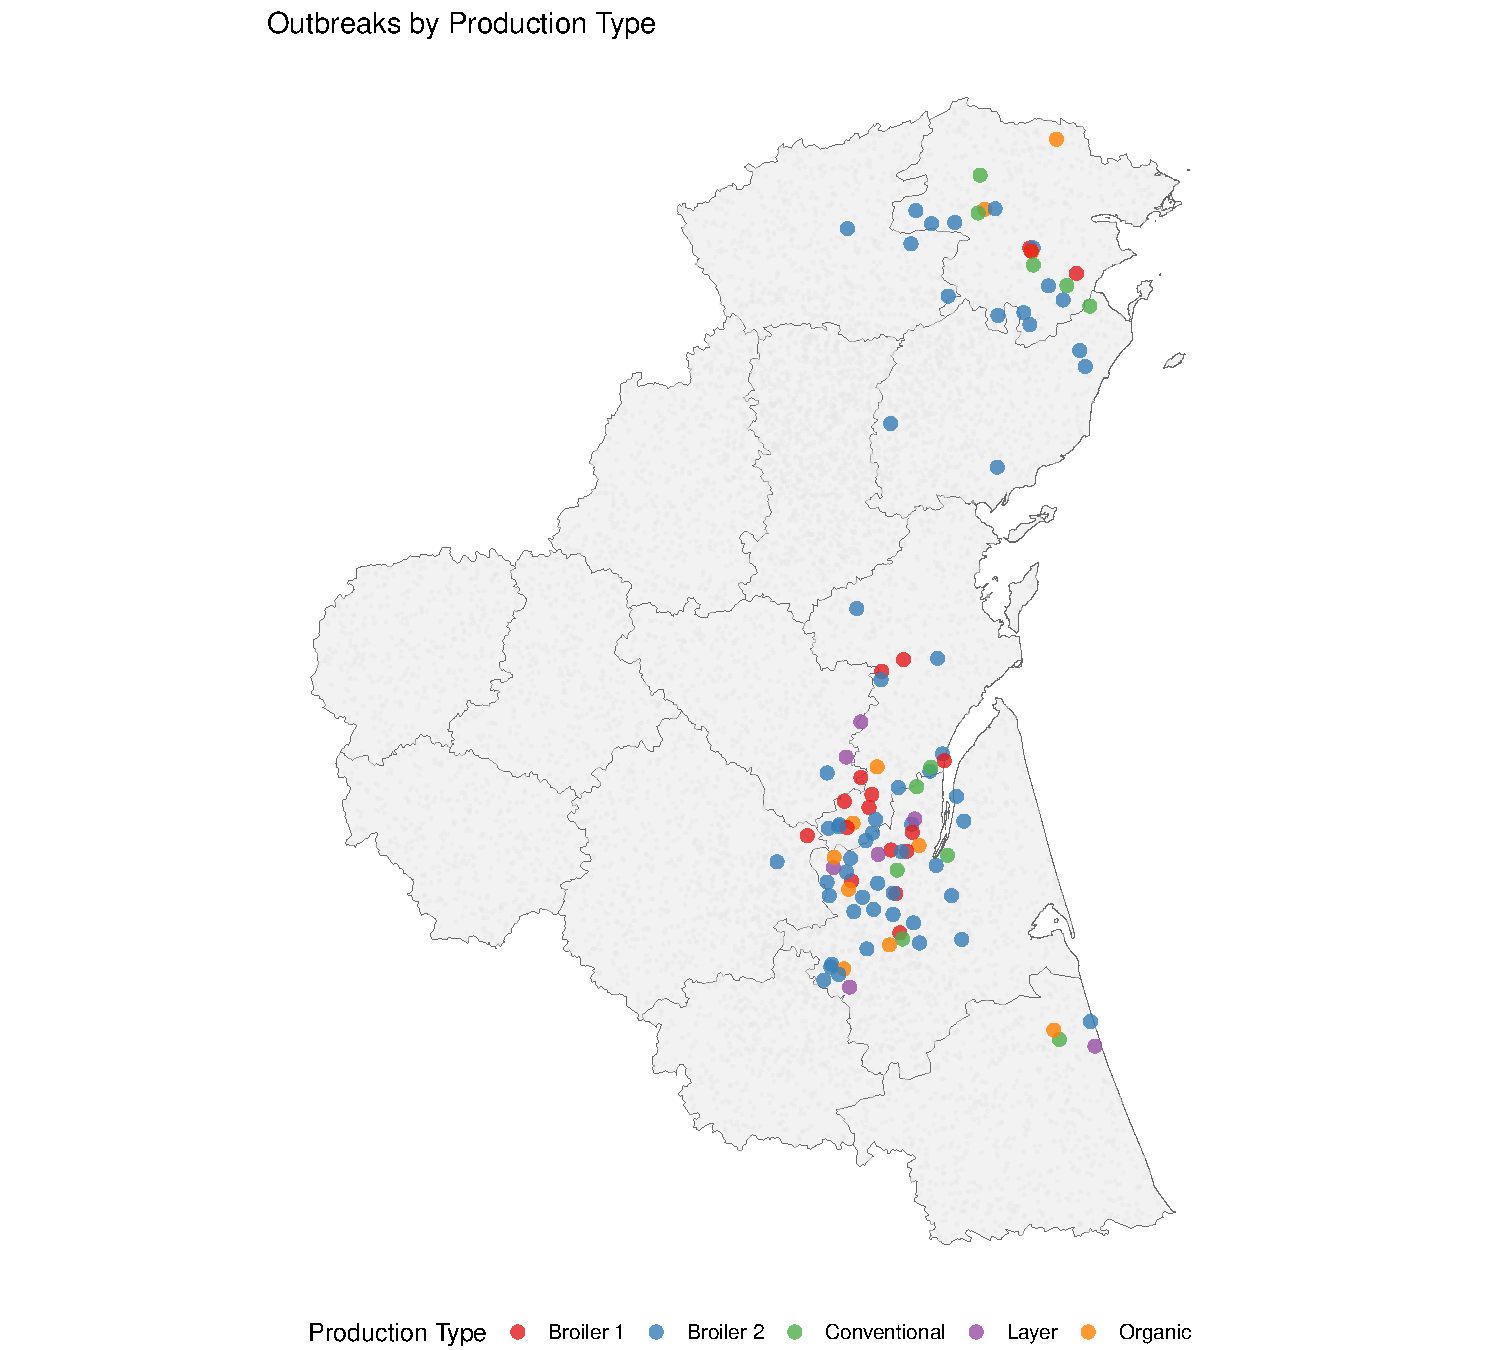
\includegraphics[keepaspectratio]{phase-1-q-1_files/figure-pdf/fig-map-production-1.pdf}}

}

\caption{\label{fig-map-production}Spatial distribution of outbreaks
coloured by production type.}

\end{figure}%

\section{Movement Network}\label{movement-network}

The movement dataset records \textbf{7,187 animal movements} between
3,994 farms from September 01, 2025 to January 13, 2026. The network has
a directed structure: \textbf{1,248 source farms} (all broiler\_1) ship
to \textbf{2,746 destination farms} (all broiler\_2). This represents a
broiler supply chain. Duck farms (conventional and organic) are entirely
absent from the movement records.

\subsection{Network summary}\label{network-summary}

\begin{longtable}[t]{lr}

\caption{\label{tbl-movement-summary}Movement network summary
statistics.}

\tabularnewline

\toprule
Metric & Value\\
\midrule
Total movements recorded & 7,187\\
Date range & Sep 01, 2025 – Jan 13, 2026\\
Unique source farms (all broiler 1) & 1,248\\
Unique destination farms (all broiler 2) & 2,746\\
Total farms in network & 3,994\\
\addlinespace
Case farms in network & 74 of 103\\
— as source (broiler 1) & 18\\
— as destination (broiler 2) & 56\\
\bottomrule

\end{longtable}

\subsection{Movement volume over time}\label{movement-volume-over-time}

\begin{figure}

\centering{

\pandocbounded{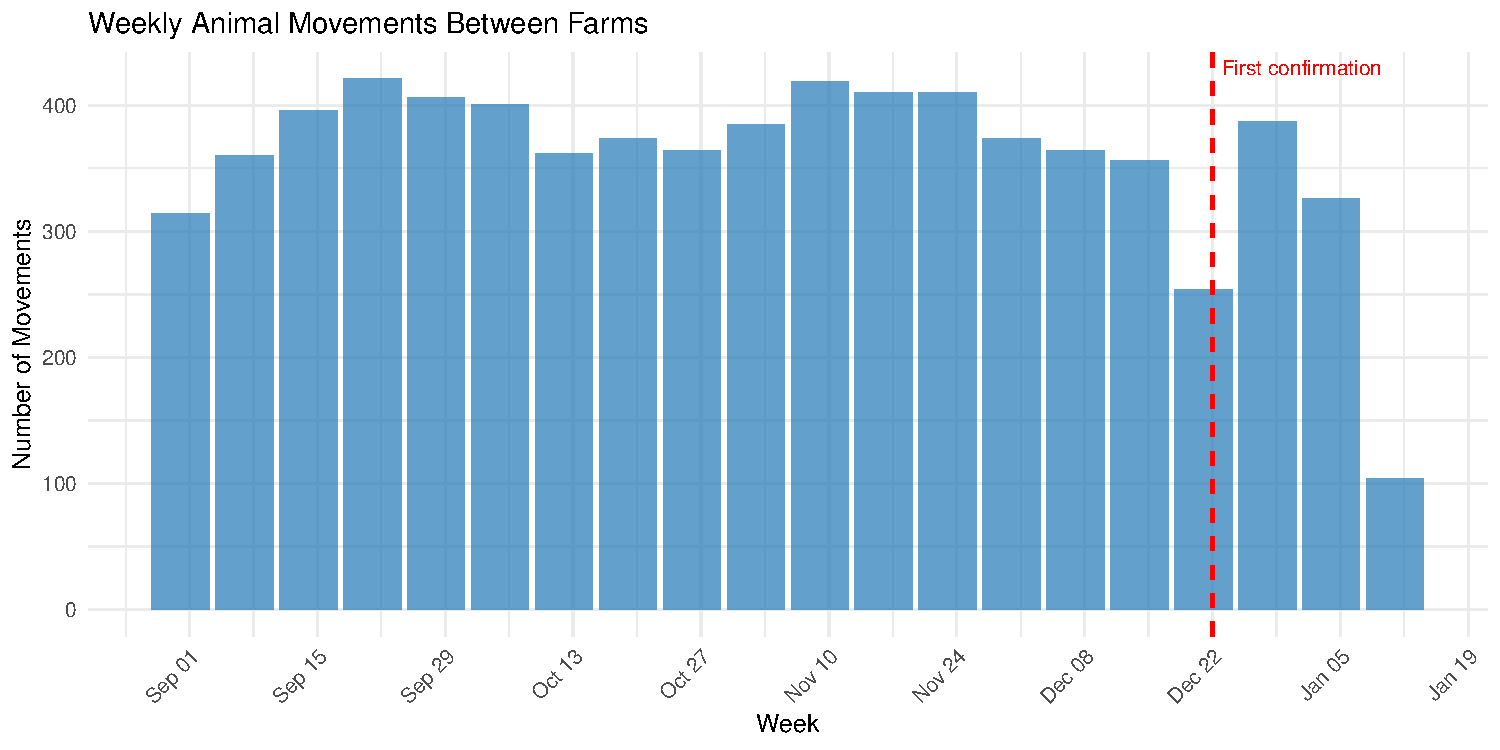
\includegraphics[keepaspectratio]{phase-1-q-1_files/figure-pdf/fig-movement-volume-1.pdf}}

}

\caption{\label{fig-movement-volume}Weekly movement volume. The vertical
dashed line marks the date of the first confirmed outbreak (December 22,
2025). Movement volumes decline during the outbreak period.}

\end{figure}%

\subsection{Case farm involvement}\label{case-farm-involvement}

\begin{longtable}[t]{lr}

\caption{\label{tbl-case-movements}Movements involving confirmed case
farms: timing relative to confirmation and direct case-to-case links.}

\tabularnewline

\toprule
Metric & Count\\
\midrule
Movements FROM case farms & 88\\
— before confirmation & 85\\
— on day of confirmation & 3\\
— after confirmation & 0\\
Movements TO case farms & 165\\
\addlinespace
— before confirmation & 165\\
Direct case → case movements & 3\\
\bottomrule

\end{longtable}

\subsection{Network visualisation}\label{network-visualisation}

\begin{figure}

\centering{

\pandocbounded{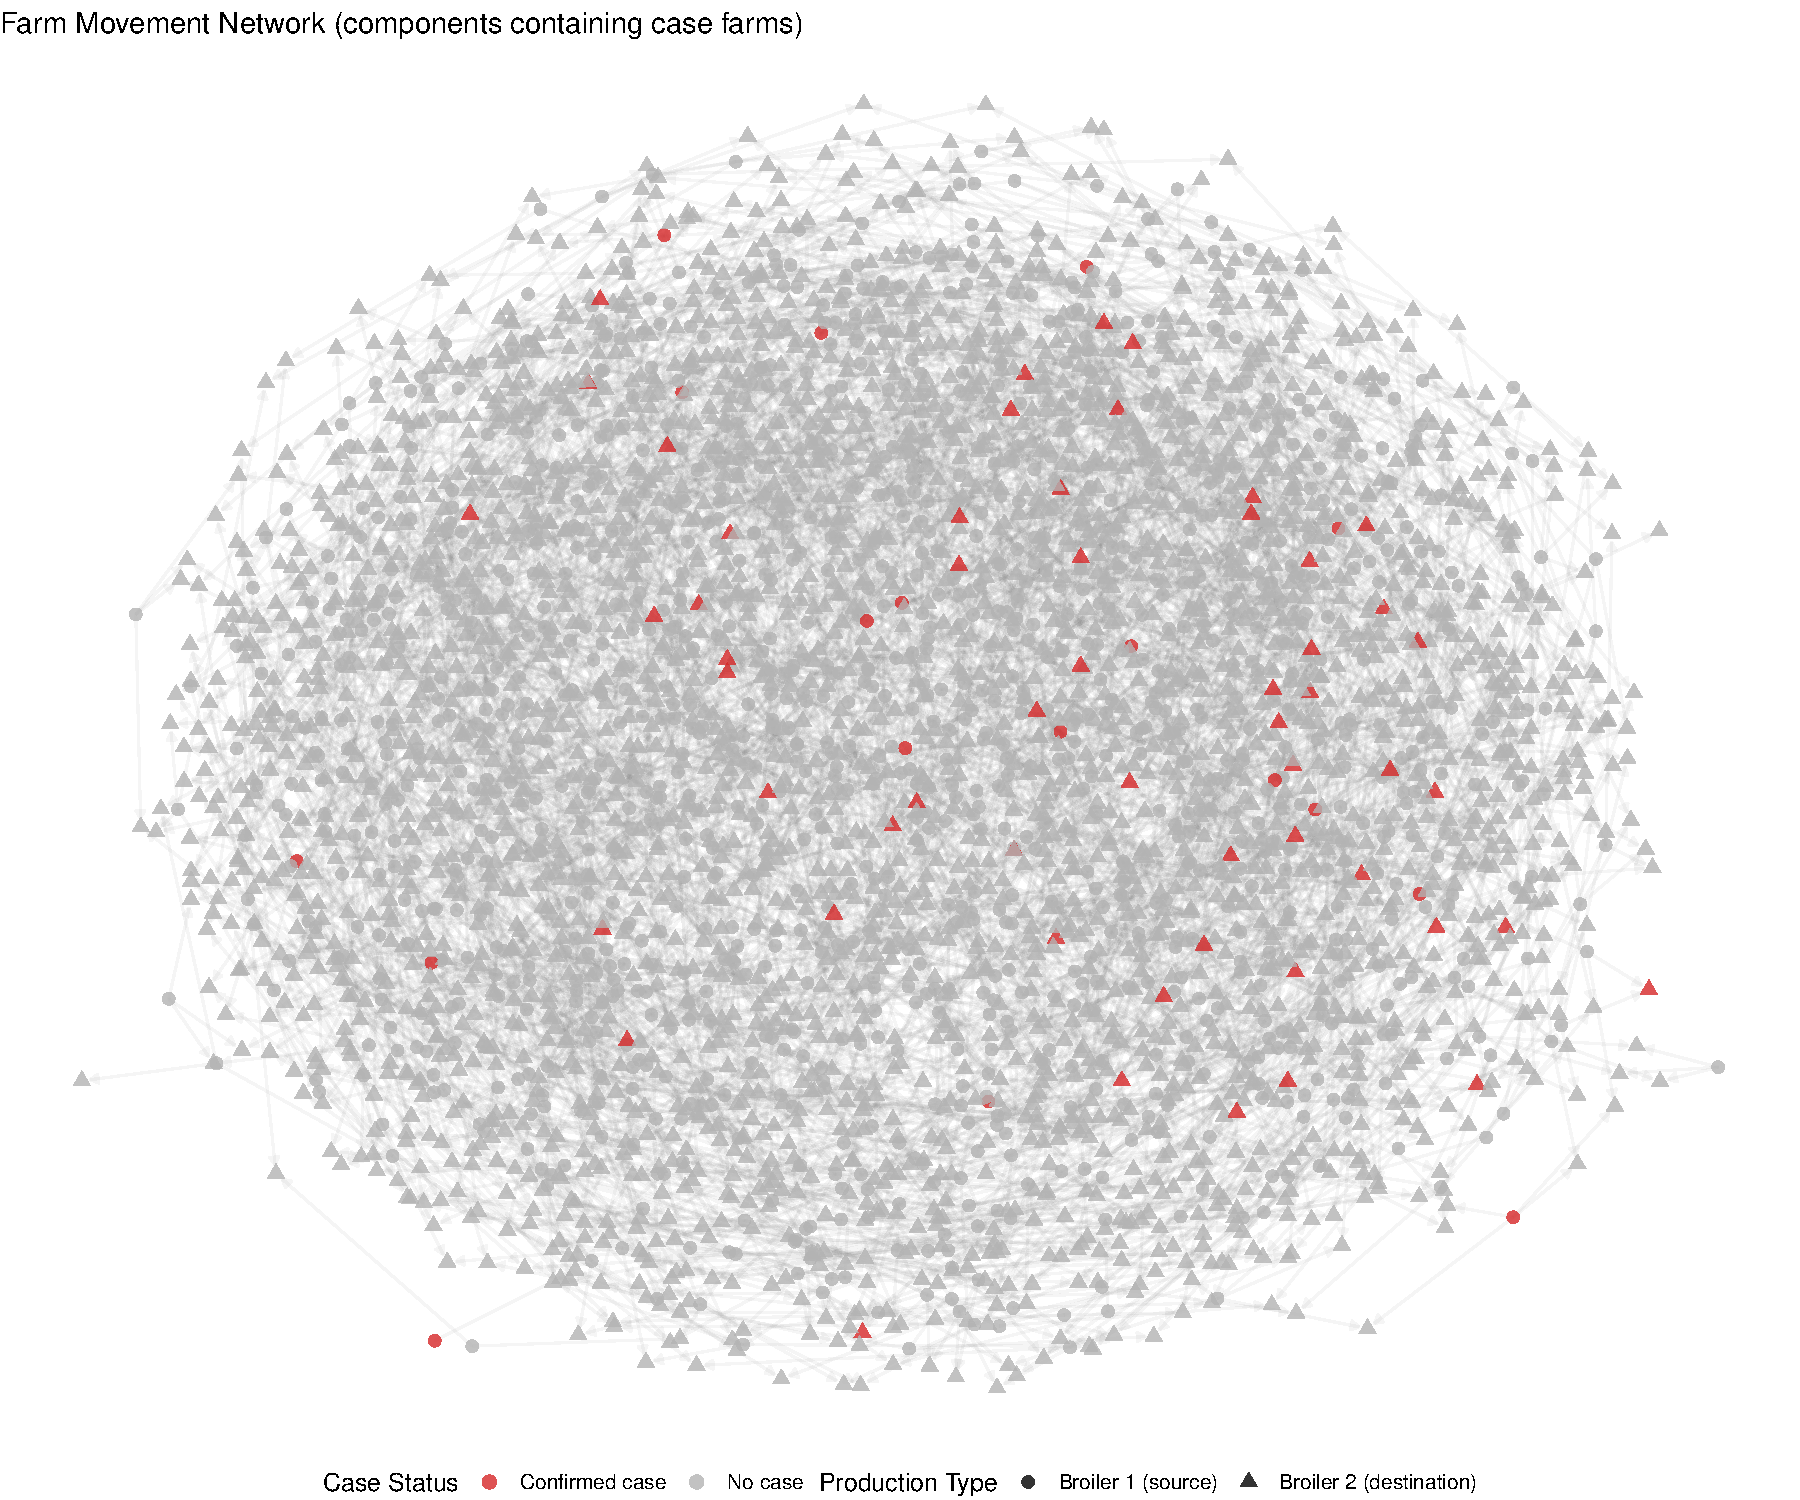
\includegraphics[keepaspectratio]{phase-1-q-1_files/figure-pdf/fig-network-1.pdf}}

}

\caption{\label{fig-network}Movement network graph. Nodes represent
farms; edges represent recorded movements (aggregated). Node colour
indicates case status; node shape indicates production type (broiler 1 =
circle, broiler 2 = triangle). Only the connected component containing
at least one case farm is shown to reduce visual clutter.}

\end{figure}%

\begin{center}\rule{0.5\linewidth}{0.5pt}\end{center}

\section{Questions arising from the
data}\label{questions-arising-from-the-data}

The descriptive patterns above raise several questions for further
investigation:

\begin{itemize}
\item
  \textbf{Is the epidemic accelerating, stabilising, or decelerating?}
  The weekly incidence table and epidemic curve provide a basis for this
  assessment. Growth rate estimation (e.g., doubling time, effective
  reproduction number) would quantify the trajectory more precisely ---
  see the companion temporal analysis for these estimates.
\item
  \textbf{Why are chicken farms, particularly broiler type 2,
  disproportionately affected?} Attack rates differ substantially across
  species and production types. Possible explanations include spatial
  confounding (chicken farms may be concentrated near the outbreak
  focus), differences in biosecurity practices by production type,
  differences in susceptibility or clinical presentation affecting
  detection probability, or transmission via production-specific supply
  chains. Disentangling these requires spatial risk factor analysis.
\item
  \textbf{Does the broiler supply chain explain the concentration of
  cases in broiler 2 farms?} The movement network is a directed broiler
  1 → broiler 2 supply chain. Broiler 2 farms have the highest attack
  rate and receive animals from broiler 1 farms, some of which are also
  confirmed cases. However, only 3 direct case-to-case movements were
  recorded. Further analysis could quantify whether farms with more
  incoming movements, or movements from case farms specifically, had
  higher infection risk --- controlling for spatial proximity.
\item
  \textbf{Is passive surveillance sufficient?} The overwhelming majority
  of detections are through passive surveillance (clinical suspicion).
  The low contribution of preshipment testing and contact tracing raises
  the question of whether subclinical or early-stage infections are
  being missed, and whether the true extent of the epidemic is larger
  than confirmed cases suggest.
\item
  \textbf{Are culling operations keeping pace with new detections?} The
  cull status data show a growing backlog of planned and in-progress
  culls. Whether delays in depopulation are contributing to onward
  transmission is a question for operational and transmission modelling.
\item
  \textbf{Where is the epidemic likely to spread next?} The
  temporal-spatial progression suggests outward expansion from an
  initial focus. Identifying the leading edge and farms at highest risk
  of future infection would inform targeted surveillance and preventive
  measures.
\end{itemize}

\section{Limitations and analytical
choices}\label{limitations-and-analytical-choices}

\subsection{Data not included in this
report}\label{data-not-included-in-this-report}

\begin{itemize}
\item
  \textbf{Mortality ledger data}: Individual farm mortality records (PDF
  format) are available for a subset of farms. These could provide
  insight into within-farm dynamics and time from infection to
  detection, but were not incorporated here.
\item
  \textbf{Preventive culls}: Data on 52 preventive culling events are
  available (\texttt{prev\_culls.csv}) but not presented, as the focus
  here is on confirmed outbreaks rather than control measures.
\item
  \textbf{Farm activity data}: Production activity logs
  (\texttt{activity.csv}) could contextualise which farms were actively
  stocked at the time of the outbreak, but were not used in this
  descriptive analysis.
\item
  \textbf{High-risk zone and wetland layers}: Geospatial data on the
  designated high-risk zone (\texttt{hrz\_32626.geojson}) and
  wetland/water body coverage (\texttt{clc\_32626.geojson}) are
  available and could add context to the spatial maps, but were omitted
  to keep the maps focused on outbreak distribution.
\end{itemize}

\subsection{Analytical limitations}\label{analytical-limitations}

\begin{itemize}
\item
  \textbf{Attack rates are crude}: The attack rates presented use total
  registered farms as the denominator. Not all farms may have been
  actively stocked during the outbreak period, so true attack rates
  among at-risk farms may differ.
\item
  \textbf{No adjustment for spatial confounding}: Differences in attack
  rates across species and production types may be partly or wholly
  explained by the geographic concentration of the outbreak rather than
  true biological differences.
\item
  \textbf{Epidemic curve right-truncation}: The most recent days of the
  epidemic curve are likely incomplete due to delays between suspicion
  and confirmation. The apparent case count in the final days may
  underestimate the true incidence.
\item
  \textbf{Movement network is descriptive only}: The movement section
  presents network structure and case involvement but does not model
  whether movements are associated with infection risk. Temporal
  precedence (movements before confirmation) does not establish
  causation. The network also only covers chicken broiler farms, so
  transmission pathways for duck and layer farms remain unobserved.
\item
  \textbf{No formal statistical testing}: This report is purely
  descriptive. Differences in attack rates have not been tested for
  statistical significance, and no regression or spatial modelling has
  been applied.
\end{itemize}




\end{document}
